\documentclass[12pt, a4paper]{article}
\usepackage{caption}
\usepackage{graphicx}
\usepackage{listings}
\usepackage{siunitx}
\usepackage{hyperref}
\def\checkmark{\tikz\fill[scale=0.4](0,.35) -- (.25,0) -- (1,.7) -- (.25,.15) -- cycle;}
\usepackage{tikz-network}
\hypersetup{
    colorlinks,
    citecolor=black,
    filecolor=black,
    linkcolor=black,
    urlcolor=black
}
\usepackage{amsmath, amsfonts, amssymb, amsthm}
\usepackage{algpseudocode}
\usepackage{algorithm}
\renewcommand{\thesubsubsection}{\thesubsection.\alph{subsubsection}}
\title{Algorithms and datastructures\\Exercises}
\date{2022}
\author{Kristoffer Klokker}
\begin{document}
	\maketitle
	\clearpage
	\tableofcontents
	\clearpage
		\setcounter{section}{4}
		\section{Week}
			\subsection{For each function $f(n)$ and time $t$ in the following table, determine the alrgest size $n$ of a problem that can be solved in time $t$, assuming that the algorithm to solve the problem takes $f(n)$ 1 nanosecond}
				\begin{table}[h!]
					\begin{tabular}{|l|l|l|l|l|}
					\hline
							& 1s 			& 1hour			& 1year			& 1 centuray                              	\\ \hline
					$n$    		& $10^9$ 		& $6\cdot 10^{10}$	& $3.2\cdot 10^{16}$	& $3.2\cdot 10^{18}$ 		\\ \hline
					$n \log_2 n$	& $4\cdot 10^7$	& $10^9\frac{1}{\text{s}}\cdot 3600\text{s}=n\cdot \log_2(n)\rightarrow n=  9.8\cdot10^{10}$  & $6.4\cdot 10^{14}$ & $5.6\cdot 10^{16}$                            \\ \hline
					$n^2$      	& $31622$		& $1.8\cdot 10^6$		& $1.7\cdot 10^8$		& $1.8\cdot 10^9$			\\ \hline
					$n^3$       	& $10^3$		& $15326$			& $316010$			& $1.4\cdot 10^6$                       \\ \hline
					$2^n$       	& 30 			& $41.7$			& $54.8$			& $61.5$			           \\ \hline
					\end{tabular}
				\end{table}	
			\subsection{Show that in a puzzle where two peices is switched with $n$ pieces in all wrong positions, it requires at minimum of $n/2$ switches to solve the puzzle}
				For a puzzle with no correct positions in advance, the lowest amounts of move will be in the scenario where every piece's correct position has to piece of its current position. Which therefore will result in $n/2$ amounts of moves is needed.
			\subsection{Create a puzzle with 4 pieces, and find a sequence of switches, but where not every switch moves at least one piece to its correct position}
				\begin{table}[h!]
					\begin{tabular}{|l|l|}
					\hline
					4&1\\\hline
					2&3\\\hline
					\end{tabular}
				\end{table}	
				$4\rightarrow 2,3\rightarrow 2, 1\rightarrow 2$\\
				As seen here this method does no use the greedy method but it still use the same amount of moves.
			\subsection{Create an algorithm which can find cycles in a given puzzle}
				The algorithm takes a list, and creates a variable counter for the amount of cycles.\\
				It then goes through every entry, if the entry is not -1 then it calls a recursive function with the entry index and list.\\
				The list then check if the given entry is -1 if not then set the entry to -1 and then calls itself with the entries last index and the list.\\
				When the function returns it add 1 to the cycle.\\
				Then it returns the amount of cycles\\
				This algorithm will run at $O(2n)$ if the cycle is 1 and it then has to move every entry and go through the rest of the list. 
			\subsection{Use the algorithm implementation to calculate statistic over the amount of cycles in a 16 long permutation}
				\begin{figure}[h!]
					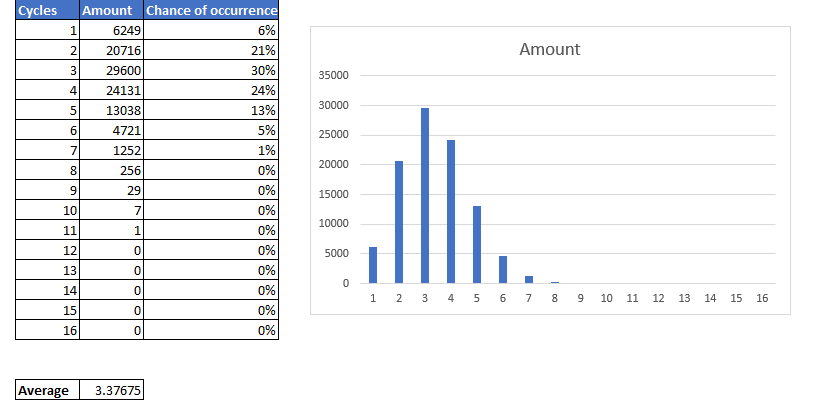
\includegraphics[width=\linewidth]{assets/week5Exercise2.png}
					\caption{Statistic from puzzleSolve/data.csv}
				\end{figure}
			\subsection{Write insertion sort pseudo code}
				\begin{algorithmic}[1]
					\State Linear search($A,v$)
					\State $i=0$
					\While{$i<A.length$ \&\& $A[i]!=v$} 
						\State $i++$
					\EndWhile
					\State return $i$
				\end{algorithmic}
		\section{Week}
			\subsection{What is the average and worst case run time og linear search aglorithm with the element placed randomly}
				Average: on average the run time will be $n/2$ \\
				Worst: if the element is at the end of the list it will be $n$
			\subsection{Let an inversion be that in an array if $i<j$ and $A[i]>A[j]$}
				\subsubsection{Find inversion pairs in $\{2,3,8,6,1\}$}
					$(2,1),(3,1),(8,1),(8,6),(6,1)$
				\subsubsection{For which array will it have the most inverse pairs and how many in an array of length $n$}
					The backwards sorted array, which will have $\frac{n^2-n}{2}$ pairs.
				\subsubsection{What is the relation between inversion pairs and insertion sort}
					The relation is that insertion sort use the same amount of operations in the worst case scenario as inverse pairs.
			\subsection{Analyse the run time of insertion sort, in best case, worst case and random case}
				Here 1000 arrays was used from which random length of arrays was used. Here the are the results of the time divided by length average.\\
				\begin{itemize}
					\item Best - $4.31\cdot 10^{-6}$
					\item Worst - $0.016$
					\item Random - $0.008$
				\end{itemize}
				As seen the random is closest to the worst case. 
			\subsection{Find an algorithm which for a array with integers if there exists a pair which sum is equal to $x$}
				This is done by using a sort like merge sort which takes $n\cdot \log_2n$ then two pointers where one is at the start and one at the end.\\				
				If the two pointers integer sum exceeds $x$ the end moves to the left if less than $x$ the start pointer moves to the right.\\
				This will take $n$ time and therefore the time will still just be $O(n\cdot \log_2n)$
			\subsection{Illustrate merge sort using the array $A=\{3,41,52,26,38,57,9,49\}$}
				\begin{figure}[h!]
					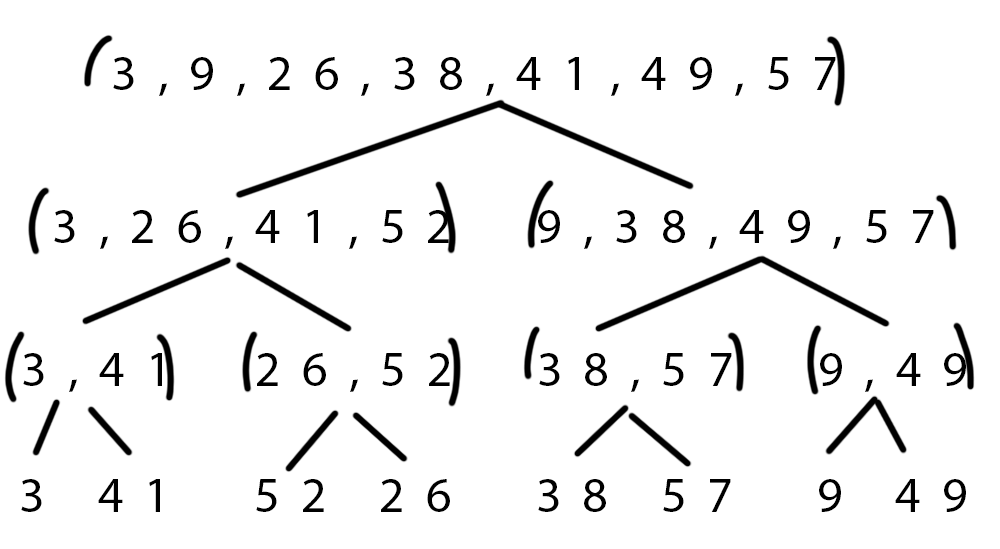
\includegraphics[width=\linewidth]{assets/week6Exercise1.png}
					\caption{Illustration of merge sort}
				\end{figure}
			\subsection{Show that for $f(n)=0.1n^2+5n+25$ that $f(n)=\Theta(n^2)$ and $f(n)=o(n^3)$}
				\begin{align*}
					\lim\limits_{n\rightarrow \infty}\frac{0.1n^2+5n+25}{n^2}=0.1\\
					\lim\limits_{n\rightarrow \infty}\frac{0.1n^2+5n+25}{n^3}=0
				\end{align*}
				Due to the first begin bigger than 0 it means that $f(n)=\Theta(n^2)$ and due to the other being zero means that $f(n)=o(n^3)$
			\subsection{Prove that $max(f(n),g(n))=\Theta(f(n)+g(n))$}
				Due to the max function the highest resullt $g(n)$ can maximally be equal to $f(n)$.\\
				Therefore if $f(n)=n^2$ $g(n)$ can maximally be $n^2$ and therefore the addition will result in the same run time.
			\subsection{Draw binary search, write pseudo code and then code}
				\begin{figure}[h!]
					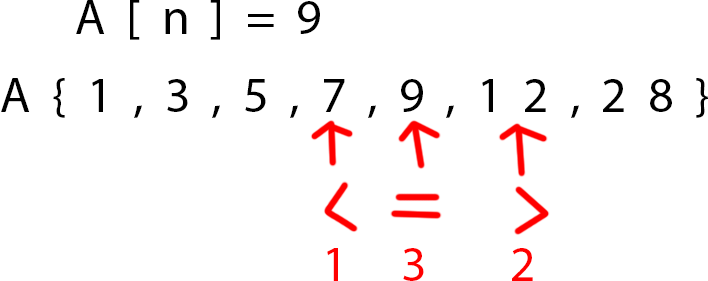
\includegraphics[width=\linewidth]{assets/week6Exercise8.png}
					\caption{Illustration of binary search}
				\end{figure}
				\begin{algorithmic}[1]
					\State Binary search($A,v$)
					\State $i=A.length/2$
					\State $j = A.length/2 + A.length\%2$
					\While{$iA[i]!= v$ $||$ $j==0$} 
						\State $j = j/2 + j\%2$
						\If{$A[i] < v$}
							\State $i = i + j$
						\Else
							\State $i = i - j$
						\EndIf
					\EndWhile
					\State return $i$
				\end{algorithmic}
			\subsection{How can binary search be used to optimize linear search to $O(n\log_2n)$?}
				By instead of linearly going down and finding a number which the current is lower than, a binary search can be done to a number which is lower.\\
				By this every entry will be performed a binary search upon an such the run time will be $n\log_2n$
			\subsection{Is $2^{n+1}=O(2^n)$? Is $2^{2n}=O(2^n)$?}
				$2^{n+1}=2^n\cdot 2^1$ therefore $2^{n+1}=O(2^n)$\\	
				$\lim\limits_{n\rightarrow \infty}\frac{2^n}{2^{2n}}=0$ therefore $2^n=o(2^{2n})$
			\subsection{Prove $\log(n!)=\Theta(n\log n)$}
				$\lim\limits_{n\rightarrow \infty}\frac{\log(n!)}{n\log(n)}=1$ therefore $\log(n!)=\Theta(n\log n)$
			\subsection{Prove $n!=\omega (2^n)$}
				$\lim\limits_{n\rightarrow \infty}\frac{2^n}{n!}=0$ therefore $2^n = o(n!) \rightarrow n!=\omega (2^n)$				
			\subsection{Prove $n!=o(n^n)$}
				$\lim\limits_{n\rightarrow \infty}\frac{n!}{n^n}=0$ therefore $n! = o(n^n) $	
		\section{Week}
			\subsection{Rank the function speed from fastest growing to slowing}
				$$\sqrt{n},2^n,\log_{10}^2n,\log_2n$$
				$\lim\limits_{n\rightarrow \infty}\frac{f(x)}{g(x)}$\\
				\clearpage
				\begin{table}[h!]
					\begin{tabular}{|l|l|l|l|l|l|}
					\hline
					$g(n)\backslash f(n)$     & $\sqrt{n}$ & $2^n$    & $\log_{10}^2n$ & $n$      & $\log_2n$ \\ \hline
					$\sqrt{n}$     & 1          & $\infty$ & 0              & $\infty$ & 0         \\ \hline
					$2^n$          & 0          & 1        & 0              & 0        & 0         \\ \hline
					$\log_{10}^2n$ & $\infty$   & $\infty$ & 1              & $\infty$ & 0         \\ \hline
					$n$            & 0          & $\infty$ & 0              & 1        & 0         \\ \hline
					$\log_2n$      & $\infty$   & $\infty$ & $\infty$       & $\infty$ & 1         \\ \hline
					\end{tabular}
				\end{table}
				This can be rearranged from a clear order is made.\\
				This is therefore the order of fastest growing to slowest $2^n,n,\sqrt{n},\log_{10}^2n,\log_2n$\\
				\begin{table}[h!]
					\begin{tabular}{|l|l|l|l|l|l|}
					\hline
					$g(n)\backslash f(n)$     & $2^n$    & $n$      & $\sqrt{n}$ & $\log_{10}^2n$ & $\log_2n$ \\ \hline
					$2^n$          & 1        & 0        & 0          & 0              & 0         \\ \hline
					$n$            & $\infty$ & 1        & 0          & 0              & 0         \\ \hline
					$\sqrt{n}$     & $\infty$ & $\infty$ & 1          & 0              & 0         \\ \hline
					$\log_{10}^2n$ & $\infty$ & $\infty$ & $\infty$   & 1              & 0         \\ \hline
					$\log_2n$      & $\infty$ & $\infty$ & $\infty$   & $\infty$       & 1         \\ \hline
					\end{tabular}
				\end{table}
			\subsection{If $f_1(n)\in O(g_1(n))$ and $f_2(n)\in O(g_2(n))$ which statements is true}
				\begin{enumerate}
					\item $f_1(n)+f_2(n)\in O(g_1(n)+g_2(n))$
					\item $g_1(n)+g_2(n)\in \Omega (f_1(n)+f_2(n))$
					\item $\frac{f_1(n)}{f_2(n)}\in O(\frac{g_1(n)}{g_2(n)})$
				\end{enumerate}
				The first statement is true due to if $f_1(n)\Omega f_2(n)$ then $g_2(n)$ will simply be a constant when added to $g_2(n)$, which also account for the other way around.\\
				The seconds is true due to being the inverse of the first statement.\\
				The third is not true, in the following assignment $f_1(n)=n^2, f_2(n)=n^2,g_1(n)=n^2,g_2(n)=n^n$ in this scenario the left will go towards 1 and the other will to 0.
			\subsection{Describe an algorithm which find the number of tuples in an array which has a lower value than another element but higher index in the run time $n\log_2n$}
				This could be done with merge sort. Here when comparing two elements if an element is choosen from the array which comes first then a tuple exists with every element left in the other array.
			\subsection{Which of the following statements are true}
				\begin{enumerate}
					\item $n^2\in \Omega(n)$
					\item $n\in \Theta(n^2)$
					\item $n\log n\in o(n^2)$
					\item $\log n \in O(\sqrt{n})$
					\item $n! \in \omega (2^n)$
				\end{enumerate}
				\begin{align}
					\lim\limits_{n\rightarrow \infty}\frac{n^2}{n}=\infty\\
					\lim\limits_{n\rightarrow \infty}\frac{n^2}{n\log_2n}=\infty\\
					\lim\limits_{n\rightarrow \infty}\frac{\sqrt{n}}{\log_2n}=\infty\\
					\lim\limits_{n\rightarrow \infty}\frac{n!}{2^n}=\infty
				\end{align}
				The first statement is true according to (1) and the second is false due to (1) not being equal 1.\\
				The third is true according to (2), likewise the fourth is true according to (3)\\
				The fifth is also true according to (4).
		\section{Week}
			\subsection{Illustrate the partitioning in quick sort on the following array}
				$$A=\{13,19,9,5,12,8,7,4,21,2,6,11\}$$
				\begin{figure}[h!]
					\center
					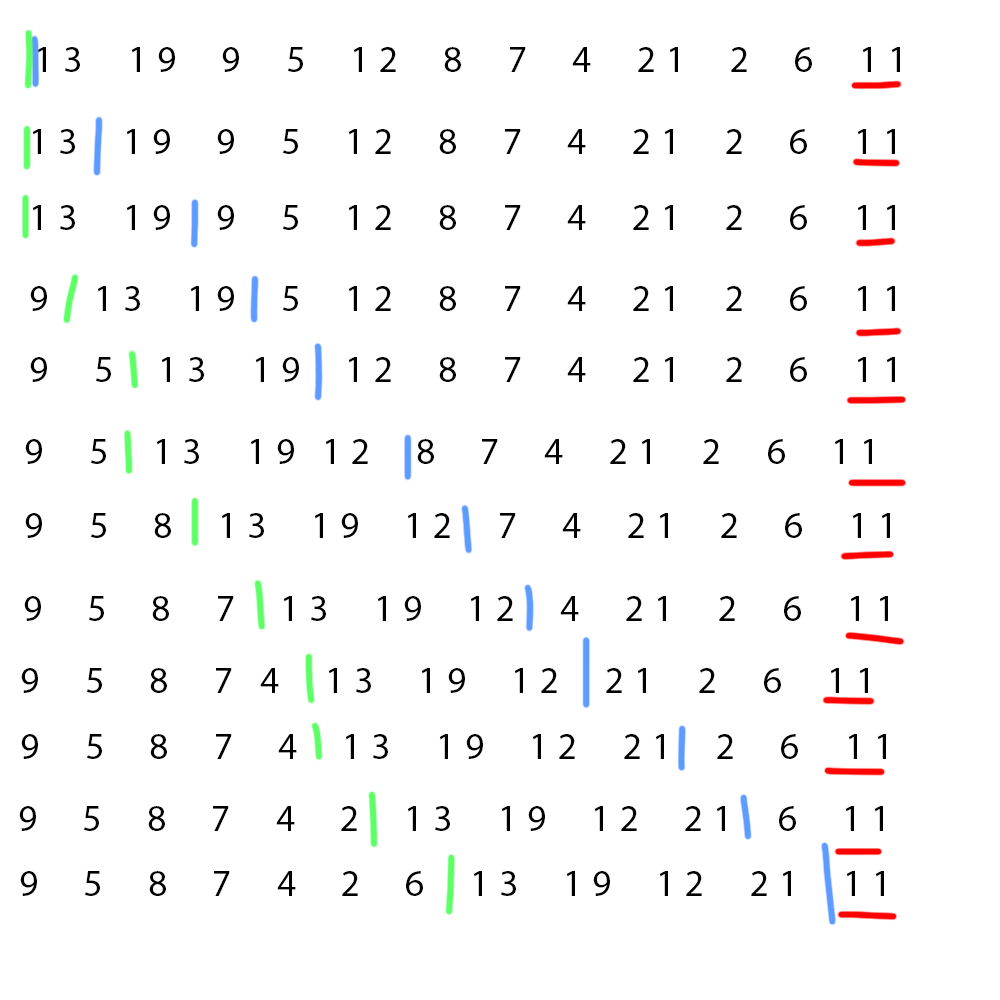
\includegraphics[width=300px]{assets/week8Exercise1.png}
					\caption{Quick sort partioning on an array}
				\end{figure}
			\subsection{In an array with only the same value, where will quick sort return the middle value}
				The returned placement will then be the length of the array -1 / the last element in the array.\\
			\subsection{What is the run time of quick sort on the  array of the same value}
				This will either be the best case or worst case for the algorithm.\\
				This is due to if left partition is $\leq$ nothing is moved. Whereas if the right partition is $\geq$ it will have to move every element.
			\subsection{Is an sorted array a min-heap}
				Yes due to in a sorted array $2i$ and $2i+1$ will always be lower or equal
			\subsection{Is the following array a max-heap?}
				$$<23,17,14,6,13,10,1,5,7,12>$$
				It is not a valid max-heap due to 6's children is 5 and 7 which is not smaller.
			\subsection{Insert 9 into the following max-heap tree}
				$$<10,8,6,3,7,4,5,1,2>$$
				by inserting it on index 3 the following tree is made\\
				$<10,8,9,3,7,4,5,1,2>$\\
				This can then be checked\\
				$10 > 8,9$\\
				$8 > 3,7$\\
				$9 > 4,5$\\
				$3 > 1,2$\\
				It is therfore a valid max-heap
			\subsection{Insert 2 into the following min-heap}
				$$<1,3,5,4,10,13,7,6,17>$$
				$<1,2,3,5,4,10,13,7,6,17>$\\
				$1 < 2,3$\\
				$2 < 5,4$\\
				$3 < 10,13$\\
				$5 < 7,6$\\
				$10 < 17$
			\subsection{Illustrate Max-Heapify($A$,2) on the following array}
				$$<27,17,3,16,13,10,1,5,7,12,4,8,9,0>$$
				$<27,17,\color{red}2\color{black},3,16,13,10,1,5,7,12,4,8,9,0>$\\
				$2 > 13, 10$\\
				$<27,17,13,16,13,\color{red}2\color{black},10,1,5,7,12,4,8,9,0>$\\
				$2 > 4, 8$\\
				$<27,17,3,16,13,8,10,1,5,7,12,4,\color{red}2\color{black},9,0>$\\
			\subsection{Use Heap-Extract-Max(A) on the following array}
				$$<21,18,10,12,8,9,4,7,5,2>$$
				$<\color{red}2\color{black},18,10,12,8,9,4,7,5,\color{blue}21\color{black}>$\\
				$<18,\color{red}2\color{black},10,12,8,9,4,7,5,\color{blue}21\color{black}>$\\
				$<18,12,10,\color{red}2\color{black},8,9,4,7,5,\color{blue}21\color{black}>$\\
				$<18,12,10,7,8,9,4,\color{red}2\color{black},5,\color{blue}21\color{black}>$\\
				$<\color{red}5\color{black},12,10,7,8,9,4,2,\color{blue}18,21\color{black}>$\\
				$<12,\color{red}5\color{black},10,7,8,9,4,2,\color{blue}18,21\color{black}>$\\
				$<12,8,10,7,\color{red}5\color{black},9,4,2,\color{blue}18,21\color{black}>$\\
				$<\color{red}2\color{black},8,10,7,5,9,4,\color{blue}12,18,21\color{black}>$\\
				$<10,8,\color{red}2\color{black},7,5,9,4,\color{blue}12,18,21\color{black}>$\\
				$<10,8,9,7,5,\color{red}2\color{black},4,\color{blue}12,18,21\color{black}>$\\
				$<\color{red}4\color{black},8,9,7,5,2,\color{blue}10,12,18,21\color{black}>$\\
				$<9,8,\color{red}4\color{black},7,5,2,\color{blue}10,12,18,21\color{black}>$\\
				$<\color{red}2\color{black},8,4,7,5,\color{blue}9,10,12,18,21\color{black}>$\\
				$<8,\color{red}2\color{black},4,7,5,\color{blue}9,10,12,18,21\color{black}>$\\
				$<8,7,4,\color{red}2\color{black},5,\color{blue}9,10,12,18,21\color{black}>$\\
				$<\color{red}5\color{black},7,4,2\color{blue}8,9,10,12,18,21\color{black}>$\\
				$<7,\color{red}5\color{black},4,2\color{blue}8,9,10,12,18,21\color{black}>$\\
				$<\color{red}2\color{black},5,4\color{blue}7,8,9,10,12,18,21\color{black}>$\\
				$<5,\color{red}2\color{black},4\color{blue}7,8,9,10,12,18,21\color{black}>$\\
				$<\color{red}4\color{black},2\color{blue}5,7,8,9,10,12,18,21\color{black}>$\\
				$<\color{red}2\color{black}\color{blue}4,5,7,8,9,10,12,18,21\color{black}>$\\
				$<\color{blue}2,4,5,7,8,9,10,12,18,21\color{black}>$\\
			\subsection{Where in a max heap will the smallest element reside}
				Due to the trees nature, a specific index is not known rather just it is at a leaf in the tree
			\subsection{Find all mini-heaps with the elements 1,2,3,4}
				$<4,3,2,1>$\\
				$<4,2,3,1>$\\
				$<4,3,1,2>$\\
			\subsection{Prove that the childrens index relative to the parent is index times two and index times two plus 1}
				For a parent the position can be divided to the sum of the current height and the index of the level.\\
				Ex the parent 13 can be written as (8+5) where 8 is the height index and 5 is the offset.\\
				The child index will then be on the next height therefore the double height index, and the offset will then be the double due to every sibling to the parent having 2 children.\\
				Therefore in the example the parents child will be 2(8+5) therefore two times index, and the other child will have the offset of plus 1.
			\subsection{Analysis if d-ary heap}
				d-ary heaps have d children instead of two
				\subsubsection{What would be the array representation}
					This would be the same but instead of children being at 2i and 2i+1 it would be 3i and 3i+1\\
				\subsubsection{What is the height of a tree with n elements with d children}
					A level consist of $3^n$ where $n$ is the height.\\
					Therefore for a level it will be the sum of all previus level.\\
					That sereis can be condensed to $\frac{3^n-1}{2}$
				\subsubsection{Rewrite heap sort such it works with d-ary heaps}
					First of when referencing the children it will be $di$ and $di+1$\\
					When moving keys around there will then be $d$ checks for the largest value.\\
					It can here be noted that hte height of the tree was $\frac{3^n-1}{2}$ therefore making the run time $O(3^n\cdot n)$ due $n$ exhanges being done at each level.
		\section{Week}
			\subsection{Show that the worst-case running time of Heapsort is $\Omega(n\log n)$}
				Heap sort is based upon the a binary tree which height with $n$ nodes will be $\log n$. Therefore in the worst case the element os moved through out the whole tree height $n$ times. Therefore making the run time $n \log n$. 
			\subsection{Illustrate counting sort}
				\begin{figure}
					\center
					\includegraphics[width=300px]{assets/Week9Exercise2.png}
					\caption{Counnting sort illustration}
				\end{figure}
			\subsection{In the following code for counting sort, will it still work if line 9 got switched such it went from 1 to $A.length$}
				\begin{algorithmic}[1]
					\State Count search($A,B,k$)
					\State C = new Array()\{0,0,0,... k times\};
					\For {$j=1$ to $A.length$}
						\State $C[A[j]]++$ 
					\EndFor
					\For {$i=1$ to $k$}
						\State $C[i] = C[i] + C[i+1]$
					\EndFor
					\For {$j= A.length$ to $1$}
						\State $B[C[A[j]]] = A[j]$
						\State $C[A[j]] = C[A[j]] -1$
					\EndFor
				\end{algorithmic}
				For it to work the element is simply out in at index $j$ the amount of times of the value of $A[j]$. This also eleminates the before hand for loop on line 6.
			\subsection{Make an algorithm which in constant time can answer amount of elements in a range, with a preprocess time of $\Theta(n+k)$}
				\begin{algorithmic}[1]
					\State CountElementsBefore($A,k$)
					\State C = new Array()\{0,0,0,... k times\};
					\For {$j=1$ to $A.length$}
						\State $C[A[j]]++$ 
					\EndFor
					\For {$i=1$ to $k$}
						\State $C[i] = C[i] + C[i+1]$
					\EndFor
					\State $ElementsInRange(A,k,s,e)$
					\State $B = CountElementsBefore(A,k)$
					\State return $B[e]-B[s]$
				\end{algorithmic}
				Here the range must be between 0 and $k$
			\subsection{Which of the following sorting algorithms are stable and unstable, and how could they be stable}
				\subsubsection{Insertion sort}
					Insertion sorts will be stable, due to the sorting starting from 0 and when moving it will move as long it is smaller but not equal.
				\subsubsection{Merge sort}
					Insertion sort will be stable, due to if elements are equal it should take form the same array and otherwise pairs will have same order.
				\subsubsection{Heapsort}
					Heap sort is not stable. A clear example is $3(a),3(b),2,1$ first $3(a)$ is choosen $3(b),2,1,3(a)$, then $3(b)$ is choosen $2,1,3(b),3(a)$.\\
					To make it stable a MIN heap sort could be used. It would get so complication in the array range, so a list would be needed or move every element.
				\subsubsection{Quicksort}
					The quick sort will be unstable due to in the case of $1,3,4,8(a),8(b),5,\color{red}7\color{black}$, when at the 5 it would be switched with $8(a)$ and therfore change the order.\\
					To make it stable to array list could be created and elements could be moved to each such that no switching in between is needed.
			\subsection{Perform radis sort on the following inputs}
				$$747,765,544,754,431,231,222$$
				\begin{center}
					COW,DOG,SEA,RUG,ROW,MOB,BOX,TAB
				\end{center}
				\subsubsection{Numbers} 
					\begin{table}[h!]
					\begin{tabular}{llllllllll}
					\cline{1-8}
					\multicolumn{1}{|l|}{747} & \multicolumn{1}{l|}{765}                          & \multicolumn{1}{l|}{754}                          & \multicolumn{1}{l|}{431}                          & \multicolumn{1}{l|}{231}                          & \multicolumn{1}{l|}{222} & \multicolumn{1}{l|}{} & \multicolumn{1}{l|}{}                                   &                       &                       \\ \cline{1-8}
					0                         & 1                                                 & 2                                                 & 3                                                 & 4                                                 & 5                        & 6                     & 7                                                       & 8                     & 9                     \\
					                          & \begin{tabular}[c]{@{}l@{}}431\\ 231\end{tabular} & 222                                               &                                                   & 754                                               & 765                      &                       & 747                                                     &                       &                       \\ \hline
					\multicolumn{1}{|l|}{431} & \multicolumn{1}{l|}{231}                          & \multicolumn{1}{l|}{222}                          & \multicolumn{1}{l|}{754}                          & \multicolumn{1}{l|}{765}                          & \multicolumn{1}{l|}{747} & \multicolumn{1}{l|}{} & \multicolumn{1}{l|}{}                                   & \multicolumn{1}{l|}{} & \multicolumn{1}{l|}{} \\ \hline
					0                         & 1                                                 & 2                                                 & 3                                                 & 4                                                 & 5                        & 6                     & 7                                                       & 8                     & 9                     \\
					                          &                                                   & 222                                               & \begin{tabular}[c]{@{}l@{}}431\\ 231\end{tabular} & \begin{tabular}[c]{@{}l@{}}754\\ 747\end{tabular} &                          & 765                   &                                                         &                       &                       \\ \hline
					\multicolumn{1}{|l|}{222} & \multicolumn{1}{l|}{431}                          & \multicolumn{1}{l|}{231}                          & \multicolumn{1}{l|}{754}                          & \multicolumn{1}{l|}{747}                          & \multicolumn{1}{l|}{765} & \multicolumn{1}{l|}{} & \multicolumn{1}{l|}{}                                   & \multicolumn{1}{l|}{} & \multicolumn{1}{l|}{} \\ \hline
					0                         & 1                                                 & 2                                                 & 3                                                 & 4                                                 & 5                        & 6                     & 7                                                       & 8                     & 9                     \\
					                          &                                                   & \begin{tabular}[c]{@{}l@{}}222\\ 231\end{tabular} &                                                   & 431                                               &                          &                       & \begin{tabular}[c]{@{}l@{}}754\\ 747\\ 765\end{tabular} &                       &                       \\ \hline
					\multicolumn{1}{|l|}{222} & \multicolumn{1}{l|}{231}                          & \multicolumn{1}{l|}{431}                          & \multicolumn{1}{l|}{754}                          & \multicolumn{1}{l|}{747}                          & \multicolumn{1}{l|}{765} & \multicolumn{1}{l|}{} & \multicolumn{1}{l|}{}                                   & \multicolumn{1}{l|}{} & \multicolumn{1}{l|}{} \\ \hline
					\end{tabular}
					\end{table}
				\subsubsection{Letters}
					\begin{table}[h!]
					\tiny
					\begin{tabular}{|l|l|l|l|l|l|l|l|l|l|l|l|l|}
					\hline
					COW & DOG                                               & SEA & ROW & MOB & BOX & TAB &                                                                     &     &     &     &                                                   &     \\ \hline
					A   & B                                                 & C   & D   & E   & G   & M   & O                                                                   & R   & S   & T   & W                                                 & X   \\
					SEA & \begin{tabular}[c]{@{}l@{}}MOB\\ TAB\end{tabular} &     &     &     & DOG &     &                                                                     &     &     &     & \begin{tabular}[c]{@{}l@{}}COW\\ ROW\end{tabular} & BOX \\ \hline
					SEA & MOB                                               & TAB & DOG & COW & ROW & BOX &                                                                     &     &     &     &                                                   &     \\ \hline
					A   & B                                                 & C   & D   & E   & G   & M   & O                                                                   & R   & S   & T   & W                                                 & X   \\
					TAB &                                                   &     &     & SEA &     &     & \begin{tabular}[c]{@{}l@{}}MOB\\ DOG\\ COW\\ ROW\\ BOX\end{tabular} &     &     &     &                                                   &     \\ \hline
					TAB & SEA                                               & MOB & DOG & COW & ROW & BOX &                                                                     &     &     &     &                                                   &     \\ \hline
					A   & B                                                 & C   & D   & E   & G   & M   & O                                                                   & R   & S   & T   & W                                                 & X   \\
					    & BOX                                               & COW & DOG &     &     & MOB &                                                                     & ROW & SEA & TAB &                                                   &     \\ \hline
					BOX & COW                                               & DOG & MOB & ROW & SEA & TAB &                                                                     &     &     &     &                                                   &     \\ \hline
					\end{tabular}
					\end{table}	
			\subsection{Tail recursive quicsort}
				The following exercises is about the following pseudo version of quicksort, which uses tail recursion.\\
				\begin{algorithmic}[1]
					\While {$p < r$}
						\State $q$ = Partition($A,p,r$)
						\State Tail-Recursive-QuickSort(A,p,q-1)
						\State p = q+1
					\EndWhile
				\end{algorithmic}
				\subsubsection{Argue that the given version works}
					This will work due to the while loop. This will work due to the while loop going to the right and the recursive call going to the left.
				\subsubsection{Describe how the stack amount could be $n$}
					This will happend just like the worst case of quick sort where the largest element is always found as the largest element.
				\subsubsection{How could the stack call be less}
					This could be done by like other quick sort optimizations where instead of going with the left most in partitioning it should take some and find the middle and use or just a random element.
		\section{Week}
			\subsection{In the following formula, what is the best sequence such its as close to $w$ when $w=7$}
				$$\sum\limits_{i=1}^{m-1}(y_{i+1}-y_i-W)^2$$
				$(10,15,20)=(15-10-7)^2+(20-15-7)^2=-2^2+(-2)^2=8$
			\subsection{Which of these are not a possible search sequence for 363 in a binary tree of 1 to 1000}
				\subsubsection{$2,252,401,398,330,344,397,363$}
					This is a valid search
				\subsubsection{$924,220,911,244,898,258,362,363$}
					This is a valid search
				\subsubsection{$925,202,911,240,912,245,363$}
					This is not a valid path due to 912 being under the smaller branch of 911
			\subsection{Write code to find the predecessor / ordered node before}
				predecessor(x)
				\begin{algorithmic}[1]
					\While {$MIN(x.p) == x$}
						\State $x = x.p$
					\EndWhile
					\State return $MIN(x.p)$
				\end{algorithmic}
			\subsection{Draw a red black tree insert of 36}
				\begin{figure}[h!]
					\center
					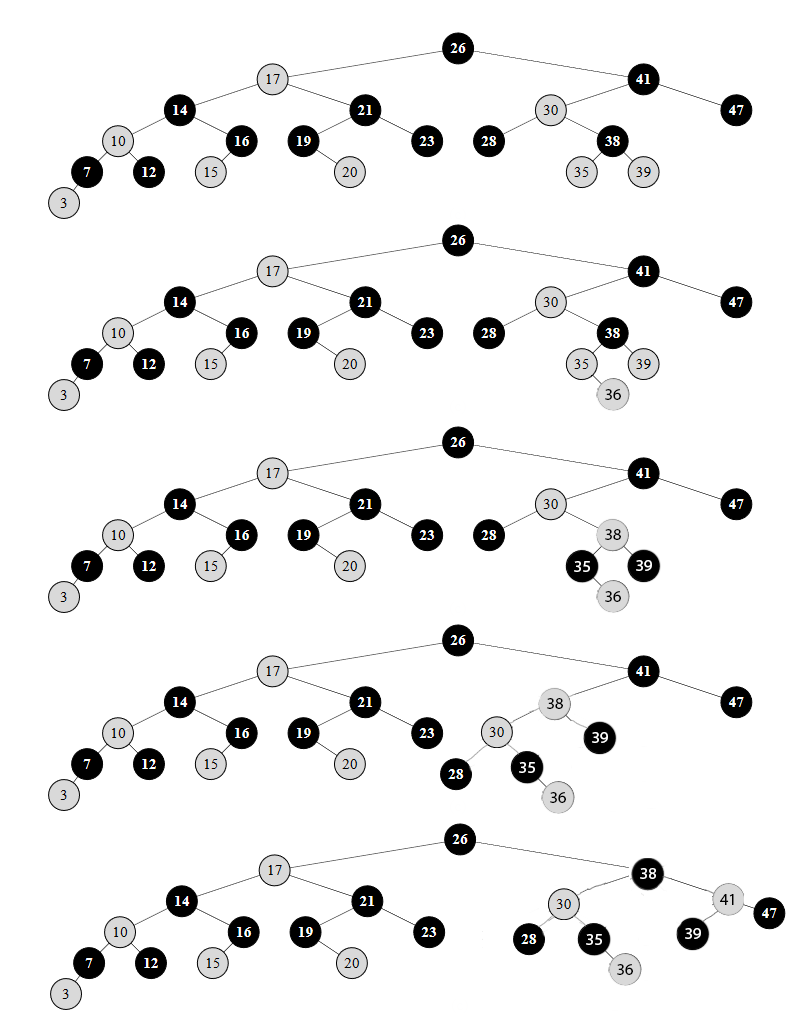
\includegraphics[width=300px]{assets/week10Exercise4.png}
					\caption{Insertion of element 36 in red-black tree}
				\end{figure}
				As seen on the figure, first it is inserted.\\
				Then uncle is red so parent, uncle and granparent change color\\
				The uncle is black and in form of triangle, the parent 30 is rotated in left direction.\\
				The uncle is black and in form of line, so parent and grandparent change color and rigt rotation on granparent.\\
			\subsection{What is the worst run time of an unbalanced tree, for a sorted list}
				In the unbalanced tree the insertion will take $n$ times by making a tree of an ordered list.\\
				The worst case will be the ordered list, where the first element is the smallest and then in an ascending order.\\
				resulting in making a list. This making of the tree wukk here take $\frac{n(n+1)}{2}$.\\
				Then the walk will then take $n$ time, making the total run time $O(n^2+n)$
			\subsection{What is the worst run time of a balanced red-black tree, for a sorted list}
				Creating the tree will take $O(n\log n)$ times, due to the height never getting over $\log n$.\\
				There when doing the walk it takes in total $O(n\log n + n)$
			\subsection{Argue that sorting $n$ elements with binary tree will take $\Omega(n\log n)$}
				A insertion will take $\log n$ time.\\
				Therefore doing that $n$ time will be $n\log n$.\\
				The walk will take $n$ but that still make the rune time $\Omega(n\log n)$
			\subsection{What is the difference between binary search tree and min-heap}
				The main difference is, that in a binary search three take for instance the root, every element to the right will always be larger than the root.\\
				Where as the min-heap is only relative to the parent which side the child i one.
			\subsection{Describe a range search for the binary tree, with the run time $\Theta(m+\log n)$}
				This is pretty simple. First a search is done for the first key, then a walk is done from there until the end range key is found.
		\section{Week}
			\subsection{Insert 18 and 26 into the given hashtable with linear opening}				
					  \begin{table}[h!]
								 \center
								 \begin{tabular}{|l|l|l|l|l|l|l|l|l|l|l|}
											\hline
											0 & 1 & 2 & 3 & 4 &5 &6 &7&8&9&10\\\hline
											67&20&17&&33&&16&2&&&15\\\hline
								  \end{tabular}
					  \end{table}
					  $$h(x)=(7x+4)\text{ mod 11}$$
					  $h(18)=130\text{ mod 11} = 9 \text{ mod 11}$\\
					  $h(26)=(186\text{ mod 11} = 10 \text{ mod 11}$\\
					  But since 10 is already in use the next linear free index is 3\\
					  \begin{table}[h!]
								 \center
								 \begin{tabular}{|l|l|l|l|l|l|l|l|l|l|l|}
											\hline
											0 & 1 & 2 & 3 & 4 &5 &6 &7&8&9&10\\\hline
											67&20&17&26&33&&16&2&&18&15\\\hline
								  \end{tabular}
					  \end{table}	
			\subsection{Insert 5,28,19,15,20,33,12,17,10 into a hash table with 9 slots and $h(x)=x$ mod 9, as a chain}
				\begin{table}[h!]
					  \center
					  \begin{tabular}{|l|l|l|l|l|l|l|l|l|}
								 \hline
								 0 & 1 & 2 & 3 & 4 &5 &6 &7&8\\\hline
									&10,19,28&20&12&&5&15,33&&17\\\hline
						\end{tabular}
				\end{table}
			\subsection{Perform hashing function on 10,22,31,4,15 with linear,quadratic, and double hashing, on mod 11 table}
					\begin{table}[h!]
					  \center
					  \begin{tabular}{|l|l|l|l|l|l|l|l|l|l|l|}
								 \hline
								 \multicolumn{11}{|c|}{Linear hash}\\
								 \hline
								 0 & 1 & 2 & 3 & 4 &5 &6 &7&8&9&10\\\hline
								 22&&&&4&15&&&&31&10\\\hline
						\end{tabular}
				\end{table}
				\begin{table}[h!]
					  \center
					  \begin{tabular}{|l|l|l|l|l|l|l|l|l|l|l|}
								  \hline
								  \multicolumn{11}{|c|}{Quadratic (c=2) hash}\\
								 \hline
								 0 & 1 & 2 & 3 & 4 &5 &6 &7&8&9&10\\\hline
								 22&&&&4&15&&&&31&10\\\hline
						\end{tabular}
				\end{table}
				\begin{table}[h!]
					  \center
					  \begin{tabular}{|l|l|l|l|l|l|l|l|l|l|l|}
								 \hline
								 \multicolumn{11}{|c|}{Double hash}\\
								 \hline
								 0 & 1 & 2 & 3 & 4 &5 &6 &7&8&9&10\\\hline
								 22&&&&4&&&&15&31&10\\\hline
						\end{tabular}
				\end{table}
		\section{Week}
			\subsection{In a tree which stores the number of children, how to find the $i$ successor to a node?}
				This would just require to find the index of the node with $OS-Rank$ and then subtract $i$ and perform a $OS-Select$ to find the successor.
			\subsection{Find the number of occurences of $i < j$ and $A[i] > A[j]$ in a given array in $O(n \log n)$}
				This can be done using an order statistic tree.\\
				The number of inversion for an element must be the elements currents index - the correct index.\\
				The correct index can be found in $O(\log n)$ time using order statistic tree and this is done for each element so $n$ times.\\
				Therefore to find the sum of all inversion occurences it will take $O(n \log n)$
			\subsection{For the following factorial code which invariants are true}
				Factorial($n$)
				\begin{algorithmic}[1]
					\State $i = n$
					\State $r = 1$
					\While {$i > 1$}
						\State $r = r * i$
						\State $ i--$
					\EndWhile
					\State return $r$
				\end{algorithmic}
				 \begin{itemize}
				 	\item $i\leq 1$ - true
				 	\item $r = i!$ - not true
				 	\item $r! \cdot i! = n!$ - not true
				 	\item $r = n!/i!$ - true
				 	\item $r=n!$ - not true
				\end{itemize}
				This can all be confirmed by the example $n=5,r=20,i=3$ which is a given state in the algorithm.
			\subsection{Solve the recursion using the master theorum}
				\subsubsection{$T(n)=4\cdot T(n/3)+n$}
					It is seen that $f(n)=O(n^{\log_3(4)})$ so the run time is $T(n)=\Omega (n^{\log_3(4)})$
				\subsubsection{$T(n)=T(n/2)+n^2$}
					$f(n)=\Omega(n^{\log_2(1)+\epsilon})$ where $0 < \epsilon < 1$\\
					run time: $T(n)=\Theta(f(n))=\Theta(n^2)$
				\subsubsection{$T(n)=16\cdot T(n/2)+n^4+n^2$}
					$f(n)=\Theta(n^{\log_2(16)})=\Theta(n^4)$\\
					run time: $T(n)=\Theta(n^{\log_2(16)}\cdot \log n)=\Theta(n^4 \log n)$
		\section{Week}
			\subsection{Solve the recursion using the master theorum}
				\subsubsection{$T(n)=2\cdot T(n/4)+1$}
					$f(n)=\Omega(n^{\log_4(2)-\epsilon})$ where $0 < \epsilon < 1$\\
					$f(n)=\Omega(n^{0.5})=\omega(\sqrt{n})$\\
					Therefore $T(n)=\Theta(\sqrt{n})$
				\subsubsection{$T(n)=2T(n-1)+n$}
					This can not be done with the master theorem.\\
					It can be seen in the tree the layers will be:\\
					$n$\\
					$2\cdot (n-1)$\\
					$2^2\cdot (n-2)$\\
					$2^i\cdot (n-i)$\\
					$2^n\cdot (n-n)$\\
					Therefore the tree have a height of $2^n$ and each will have a total run time of $O(n)$ therefore the run time will be $O(2^n\cdot n)$
			\subsection{Rethink insertion sort as a recursive algorithm and find run time}
				Insertion sort recursively will first sort from $1..n-1$ and then insert $A[n]$.\\
				Therefore it will be $T(n)=(n-1)+n$ due to the insertion taking $n$ time and only 1 child being made.\\
				The tree layers will therefore be:\\
				$n$\\
				$n-1$\\
				$n-i$\\
				$n-n$\\
				Therefore the run time of each layer being $O(n)$ and the heioght is $n$ so the total run time is $O(n^2)$
			\subsection{Use strassens algorithm on the following two matrices}
				$\begin{bmatrix}1&3\\ 7&5\end{bmatrix}\begin{bmatrix}6&8\\ 4&2\end{bmatrix}$\\
				$p1=1(8-2)=6$\\
				$p2=(1+3)2=8$\\
				$p3=(7+5)6=72$\\
				$p4=5(4-6)=-10$\\
				$p5=(1+5)(6+2)=48$\\
				$p6=(3-5)(4+2)=-12$\\
				$p7=(1-7)(6+8)=-84$\\
				$\begin{bmatrix}48-10-8-12&6+8\\ 72-10&6+48-72+84\end{bmatrix}=\begin{bmatrix}18&14\\ 62&66\end{bmatrix}$
			\subsection{Find the upper and lower bound using the master theorem}
				$$T(n)=4T(n/2)+n^2\log n$$
				$\log_2(4)=0.5$ \\
				Lower bound $f(n)=\Theta(n^{0.5})$\\
				Upper bound $f(n)=\Omega( n^{0.5+4.5})$
	\section{Week}
		\subsection{Master theoreom on recursions}
			\begin{enumerate}
				\item $T(n)=2T(n/2)+1$
				\item $T(n)=3T9n/3)+n$
				\item $T(n)=4T(n/4)+n\log n$
				\item $T(n)=5T(n/5)+n^2$
			\end{enumerate}
			\subsubsection{Solve the recursions}
				For all the recursions the $\log_b(a)$ is 1.\\
				Therefore making them:
				\begin{enumerate}
					\item $T(n)=\Theta(n)$
					\item $T(n)=\Theta( n \log\cdot n)$
					\item $T(n)=\Theta(n\log \cdot n)$
					\item $T(n)=\Theta(n^2)$
				\end{enumerate}
		\subsection{True or false?}
			\begin{itemize}
					  \item 1 is $O(2)$ - true
						\item 1 is $\Omega(2)$ - true
						\item $n$ is $O(n^2)$ - true
						\item $n$ is $\Omega(n^2)$ - false
						\item $3x+2x^2+x^3$ is $\Theta(x+2x^2+3x^3)$ - true
						\item $\log n$ is $o(n/\log n)$ - true
						\item $n^{0.5}$ is $o(n/2^n)$ - false
						\item $\log n$ is $\omega(\log n)$ -false
						\item $2^n\cdot \log n$ is $\omega(2^n)$ - true
						\item $n^2/\log n$ is $O(n(\log n)^2)$ - false
			\end{itemize}
	\section{Week}
		\subsection{Create huffman tree from the following data}
			a-300, b-150, c-75, d-125, e-200, f-50, g-100\\[4mm]
			
			1000\\
			----425\\
			-------200e\\
			-------225\\
			----------125\\
			-------------50f\\
			-------------75c\\
			----------100g\\
			----575\\
			-------275\\
			----------125d\\
			----------150b\\
			-------300g
		\subsection{Describe an algorithm whihc find schedules and amount of room needed for lectures}
			This can be a greedy, it can then go through each lecture in order of the lecture starting time.\\
			Then it goes through each room at tries to see if it fits. If it fits insert it if not go to next room.\\
			This will result in the optimal solutions, due to a new lecture hall will only be opened in case of enough other lectures overlap. The solution will not be optimal packed such most lectures are after eachother but the solution will still be optimal.
		\subsection{Argue that just taking the shortest lecture will not work, what about least overlapping?}
			The first can be argued with a counter example of lecture\\
			10-13\\
			13-14\\
			10-11\\
			11-15\\
			Taking the shortest will result 3 halls and the optimal result if 2 halls.\\
			The same example shows again that the least overlapping will not work, due to the shortest overlapping the least and therefore the same order is used, such 3 halls is needed.
		\subsection{Describe an algorithm which finds the shortest span of sums between given points}
			THis would be done with greedy algorithm. By taking the points in descending order it will find the optimal solution.\\
			It will not match such every point will get the shortest possible match, but rather the sum of all will even out to be optimal.\\
			Let say in an example with the points 1,5,6,9 the optimal solution will be 1-5 and 6-9 even though 5-6 is shorter.
		\subsection{Prove that in a file of characters the huffman algorithm will not be compressed if the highest frequency is less than half of least frequent}
			For 256 characters the worst case scenario is a tree with the height of 255, therefore the least frequenct charater having a bit length of 254. The worst case tree will therefore only optimze upon 9 character which afterwards will have a bit length longer than 8. Therefore with only half a frequency more, this will mean that the saved space on the first 9 caracters will not outweight the unsaved space on the rest 245 characters even the half as frequent.
	\section{Week}
		\subsection{Show the data strcture result of the following code, using linked list}
			\begin{algorithmic}[1]
				\For{$i=1$ to $16$}
					\State Make-Set($x_i$)
				\EndFor
				\For{$i=1$ to $15$ by $2$}
					\State Union($x_i,x_{i+1}$)
				\EndFor
				\For{$i=1$ to $13$ by $4$}
					\State Union($x_i,x_{i+2}$)
				\EndFor
				\State Union($x_1,x_5$)
				\State Union($x_{11},x_{13}$)
				\State Union($x_1,x_{10}$)
				\State Find-Set($x_2$)
				\State Find-Set($x_9$)
			\end{algorithmic}
			$[x_1,x_2,x_3,x_4,x_5,x_6,x_7,x_8,x_9,x_{10},x_{11},x_{12},x_{13},x_{14},x_{15},x_{16}]$\\
			Therefore the Find-Set will both return $x_1$
		\subsection{Perform the former task as a disjoint fores using union by rank and path compression}
			This does not really change anything due to all unions and finds are called on nodes which are the first child to root anyways.
		\subsection{Find the solutions for the following recursivefunctions}
			\subsubsection{$T(n)=2T(n/3)+n$}
				$\log_3(2)\approx 0.63$\\
				$f(n)=\Omega (n^{0.64}) \rightarrow T(n)=\theta (f(n))$\\
				$T(n)=n$
			\subsubsection{$T(n)=32T(n/4)+n^{2.5}$}
				$\log_4(32)=2.5$\\
				$f(n)=\theta(n^{2,5})\rightarrow T(n)=\theta(n^{2.5}\cdot \log(n))$
		\subsection{Which of the following are true or false}
			\begin{itemize}
				\item $n^2$ is $O(n^2)$ - true
				\item $n^2$ is $\theta(n^2)$ - true
				\item $n^4$ is $O(5n^3+3n^5)$ - true
				\item $n^4$ is $\theta(5n^3+3n^5)$ - false
				\item $n\log n$ is $O(n^{1.5})$ - true
				\item $n$ is $O(\log n)$ - false
				\item $(\log n)^{10}$ is $O(n^{0.1})$ - false
				\item $1$ is $O(n)$ - true
				\item $n^2$ is $o(n^3)$ - true
				\item $n^3$ is $\omega(n^2)$ - false
			\end{itemize}
		\subsection{Perform Build-Max-Heap on the following array}
			$$[5,4,3,2,1,10,9,8,7,6]$$
			$$[10, 8, 9, 7, 6, 3, 5, 2, 4, 1]$$
		\subsubsection{Insert into the following hash array the values 3,5,15}
			The table use double hashing using the following functions:
				$$h_1(x)=(5x+1)\; mod\; 13$$
				$$h_2(x)=1+(x\; mod\;12)$$
			H:$18,\;,8,\;,\;,6,\;,\;,30,25,\;,2,23$\\
			$h_1(3)=3$\\
			H:$18,\;,8,3,\;,6,\;,\;,30,25,\;,2,23$\\
			$h_1(5)=0$\\
			$h_2(5)=8$\\
			since 8 is used, then it goes 16 mod 13 = 3 which is not open. 11 is not either, but 19 mod 13 = 6 is not.\\
			H:$18,\;,8,3,\;,6,5,\;,30,25,\;,2,23$\\
			$h_1(15)=11$\\
			$h_2(15)=4$\\
			15 mod 13 = 2, 6, 10\\
			H:$18,\;,8,3,\;,6,\;,\;,30,25,15,2,23$\\
		\subsubsection{Perform Radix-Sort(A,4) on the following array}
			$$A:[8345,7112,1830,5001,4345,2222,9112,6363]$$
			
			$A:[1830, 5001, 7112, 2222, 9112, 6363, 8345, 4345]$\\
			$A:[5001, 7112, 9112, 2222, 1830, 8345, 4345, 6363]$\\
			$A:[5001, 7112, 9112, 2222, 8345, 4345, 6363, 1830]$\\
			$A:[1830, 2222, 4345, 5001, 6363, 7112, 8345, 9112]$
		\subsubsection{Use a huffman tree on the following frequency chart, and find codes and total size of file}
			freq\\
			a:400\\
			e:750\\
			i:300\\
			o:150\\
			u:200\\
			y:100\\[4mm]
			
			Codes:\\
			a: 111\\
			e: 0\\
			u: 100\\
			y: 1010\\
			i: 110\\
			o: 1011\\
			The filesize after compression is: 4450
			
			
			
\end{document}
